\documentclass[12pt,letterpaper]{article}
\usepackage[latin1]{inputenc}
\usepackage{amsmath}
\usepackage{amsfonts}
\usepackage{amssymb}
\usepackage{graphicx}
\author{Linyun Fu}
\title{Assignment 1: Discussion of Queuing Polices}
\begin{document}
\maketitle
\part*{Question}
Consider a computer system with 10 processes in the ready queue, numbered from 0 to 9. The burst time of each process is as follows: $t_B^9=55$ ms and for $i < 9$ $t_B^i = 1.5$ ms if $i$ is an even one-digit number and $t_B^i = 3$ ms if $i$ is odd. After executing for the
burst time, each process goes into disk service that takes time $t_D$. In each question below
consider three values of $t_D$ equal to 6, 15, 25 ms, corresponding to a fast, medium and
slow disk, respectively. Assume that the disk has constant response time, regardless of
the number of processes it is serving. The context switching time $T_s$ is 1 ms.

For each question below find out a) a response time of interactive tasks (tasks with the id number other than 9), b) a slow down of the processor for the computational task
(the task numbered 9), which of course becomes infinity if this task is starving, c) the
CPU utilization. In each case consider first an abstract case in which there is no context
switching time, and then include the context switching time in your considerations.

\begin{enumerate}
\item Consider preemptive SJF scheduling for this system (also called Shortest
Remaining Time (SRT)), and use only analytical analysis to formulate your
answer (3 pts).
\item Consider HRRN scheduling (you can use either analytical analysis or emulation)
(6 pts).
\item Consider RR scheduling with time quantum $T_Q$ = 3 ms (6 pts).
\item[$\bullet$] {\bf Bonus question} worth 5 pts: include in your analysis/emulation cases of question 3, in
which time quantum, $T_Q$, is 1 ms, 1.5 ms and 11 ms, and based on these results recommend
the best value for $T_Q$ under different criteria (e.g., the CPU utilization, disk utilization, response time and slowdown).
\end{enumerate}

{\bf Clarifications:} The slowdown can be defined as the ratio of the clock time to the
execution time received by the computational process. Hence, if you emulate system to
$T_{end}$ time and during that time CPU executed the computational process for $T_{comp}$ time, then slowdown = $T_{end}/T_{comp}$.

The response time for interactive processes can be defined as the time from
entering the ready queue of the CPU till time of the request for the disk, so, the time
when a process is at the disk is not included in the response time.

The response time (like a slowdown), can become infinity if at least one of the
interactive processes is starving.

{\bf Hints:} To verify your emulator, consider FCFS algorithm first, can you provide
the answer for this case analytically? If not, see the TA during office hours.

Even more helpful could be to implement first the system discussed in class that
has only 3 processes in the ready queue. Full data for this system and a sketch of the
program for emulation are given in class.

\part*{Answer}
\section{Preemptive SJF Scheduling}
No matter what $t_D$ is, the first five processes executed would be 0, 2, 4, 6 and 8.

\subsection{$t_D=6$ ms, $T_s = 0$ ms (no context switching time)} 
In this case, Process 0 comes back to the ready queue at time point 
\begin{eqnarray}
t_B^0+t_D=1.5+6=7.5\textrm{ ms};
\end{eqnarray}
while Process 8 finishes using CPU at time point 
\begin{eqnarray}
1.5\times5=7.5\textrm{ ms};
\end{eqnarray}
so by the time Process 8 finishes using CPU, Process 0 has already come back to the ready queue, so Process 1, 3, 5, 7 and 9 suffer from starvation. Process 0, 2, 4, 6 and 8 get CPU time in turn forever.
\begin{enumerate}
\item[a)] The response times of Process 0, 2, 4, 6 and 8 are all 7.5 ms; the response times of Process 1, 3, 5 and 7 are all infinity; the average response time of all the interactive processes is infinity;
\item[b)] The slowdown of Process 9 is infinity;
\item[c)] The CPU utilization is 100\%.
\end{enumerate}

\subsection{$t_D=6$ ms, $T_s = 1$ ms (context switching time considered)} 
In this case, Process 0 comes back to the ready queue at time point
\begin{eqnarray}
T_s+t_B^0+t_D=1+1.5+6=8.5\textrm{ ms};
\end{eqnarray}
while Process 8 finishes using CPU at time point 
\begin{eqnarray}
(1+1.5)\times5=12.5\textrm{ ms};
\end{eqnarray}
so by the time Process 8 finishes using CPU, Process 0 has already come back to the ready queue, so Process 1, 3, 5, 7 and 9 suffer from starvation. Process 0, 2, 4, 6 and 8 get CPU time in turn forever.

The CPU does a 1 ms context switch and a 1.5 ms process execution in turn forever.

\begin{enumerate}
\item[a)] The response times of Process 0, 2, 4, 6 and 8 are all 12.5 ms; the response times of Process 1, 3, 5 and 7 are all infinity; the average response time of all the interactive processes is infinity;
\item[b)] The slowdown of Process 9 is infinity;
\item[c)] The CPU utilization is $1.5/(1+1.5)=60\%$.
\end{enumerate}

\subsection{$t_D=15$ ms, $T_s = 0$ ms}
In this case, Process 0 comes back to the ready queue at time point
\begin{eqnarray}
t_B^0+t_D=1.5+15=16.5\textrm{ ms};
\end{eqnarray}
while Process 8 finishes using CPU at time point 
\begin{eqnarray}
1.5\times5=7.5\textrm{ ms};
\end{eqnarray}
so by the time Process 8 finishes using CPU, Process 0 has not yet come back to the ready queue, Process 1 will be executed after Process 8, followed by Process 3 and 5. Process 5 finishes using CPU at time point
\begin{eqnarray}
7.5+3\times3=16.5\textrm{ ms};
\end{eqnarray}
so Process 0 will use CPU again, followed by Process 2, 4, 6 and 8. Process 8 finishes using CPU at time point
\begin{eqnarray}
16.5+1.5\times5=24\textrm{ ms};
\end{eqnarray}
on the other hand, Process 1 comes back to the ready queue at time point
\begin{eqnarray}
7.5+3+16=26.5\textrm{ ms};
\end{eqnarray}
so by the time Process 8 finishes using CPU, Process 1 has not yet come back to the ready queue, Process 7 will get the CPU, followed by Process 1 and 3.

The similar cycle repeats and the executing Process number is 0, 2, 4, 6, 8, 1, 3, 5, 0, 2, 4, 6, 8, 7, 1, 3, 0, 2, 4, 6, 8, 5, 7, 1, 0, 2, 4, 6, 8, 3, 5, 7, 0, 2, 4, 6, 8, 1, 3, 5, $\cdots$

The length of the cycle of execution is 

\begin{eqnarray}
(1.5\times5+3\times3)\times4=66\textrm{ ms}
\end{eqnarray}

For every 66 ms, Process 0, 2, 4, 6 and 8 finishes 4 times each, while Process 1, 3, 5 and 7 finishes 3 times each.

Process 9 cannot get any CPU time.

\begin{enumerate}
\item[a)] The response times of Process 0, 2, 4, 6 and 8 are all $66/4=16.5$ ms;
the response times of Process 1, 3, 5 and 7 are all $66/3=22$ ms;
the average response time of all the interactive processes is 
\begin{eqnarray}
(16.5\times5\times4+22\times4\times3)/(5\times4+4\times3)=18.6\textrm{ ms};
\end{eqnarray}
\item[b)] The slowdown of Process 9 is infinity;
\item[c)] The CPU utilization is 100\%.
\end{enumerate}

\subsection{$t_D=15$ ms, $T_s = 1$ ms}
In this case, Process 0 comes back to the ready queue at time point
\begin{eqnarray}
T_s+t_B^0+t_D=1+1.5+15=17.5\textrm{ ms};
\end{eqnarray}
while Process 8 finishes using CPU at time point 
\begin{eqnarray}
(1+1.5)\times5=12.5\textrm{ ms};
\end{eqnarray}
so by the time Process 8 finishes using CPU, Process 0 has not yet come back to the ready queue, Process 1 will be executed after Process 8, followed by Process 3. Process 3 finishes using CPU at time point
\begin{eqnarray}
12.5+(1+3)\times2=20.5\textrm{ ms};
\end{eqnarray}
so Process 0 will use CPU again, followed by Process 2, 4, 6 and 8. Process 8 finishes using CPU at time point
\begin{eqnarray}
20.5+(1+1.5)\times5=33\textrm{ ms};
\end{eqnarray}
Process 0 has not yet come back to the ready queue by this time, Process 5 will get the CPU, followed by Process 7, followed by Process 0, 2, 4, 6 and 8 again.

Note that we assume when two processes have the same remaining CPU time, the process that has stayed longer in the ready queue get the CPU, so although Process 1 comes back to the ready queue at time point
\begin{eqnarray}
12.5+1+3+15=31.5\textrm{ ms};
\end{eqnarray}
it still queues after Process 5 and 7, and will get the CPU right after Process 8.

The executing Process number series is 0, 2, 4, 6, 8, 1, 3, 0, 2, 4, 6, 8, 5, 7, 0, 2, 4, 6, 8, 1, 3, 0, 2, 4, 6, 8, 5, 7, $\cdots$

The length of the cycle of execution is 
\begin{eqnarray}
(1+1.5)\times10+(1+3)\times4=41\textrm{ ms}
\end{eqnarray}
For every 41 ms, Process 0, 2, 4, 6 and 8 finishes 2 times each, while Process 1, 3, 5 and 7 finishes 1 time each.

Process 9 cannot get any CPU time.

The CPU does 14 ms context switching during each cycle.

\begin{enumerate}
\item[a)] The response times of Process 0, 2, 4, 6 and 8 are all $41/2=20.5$ ms; the response times of Process 1, 3, 5 and 7 are all 41 ms; the average response time of all the interactive processes is 

\begin{eqnarray}
(20.5\times5\times2+41\times4\times1)/(5\times2+4\times1)=26.4\textrm{ ms};
\end{eqnarray}

\item[b)] The slowdown of Process 9 is infinity;
\item[c)] The CPU utilization is $(41-14)/41=65.85\%$.
\end{enumerate}

\subsection{$t_D=25$ ms, $T_s = 0$ ms}
In this case, Process 0 comes back to the ready queue at time point
\begin{eqnarray}
t_B^0+t_D=1.5+25=26.5\textrm{ ms};
\end{eqnarray}
while Process 8 finishes using CPU at time point 
\begin{eqnarray}
1.5\times5=7.5\textrm{ ms};
\end{eqnarray}
so by the time Process 8 finishes using CPU, Process 0 has not yet come back to the ready queue, Process 1 will be executed after Process 8, followed by Process 3, 5, 7 and 9. Process 9 finishes using CPU at time point
\begin{eqnarray}
7.5+3\times4+55=74.5\textrm{ ms};
\end{eqnarray}
so Process 0 will use CPU again, followed by Process 2, 4, 6, 8, 1, 3, 5 and 7. Process 7 finishes using CPU at time point
\begin{eqnarray}
74.5+1.5\times5+3\times4=94\textrm{ ms};
\end{eqnarray}
Process 9 has not yet come back to the ready queue by this time, CPU will remain idle for 5.5 ms and start executing Process 9.

The executing order is Process 0, 2, 4, 6, 8, 1, 3, 5, 7, idle for 5.5 ms, Process 9, 0, 2, 4, 6, 8, 1, 3, 5, 7, idle for 5.5 ms, Process 9, 0, 2, 4, 6, 8, $\cdots$

The length of the cycle of execution is 
\begin{eqnarray}
1.5\times5+3\times4+5.5+55=80\textrm{ ms}
\end{eqnarray}
For every 80 ms, each of the 10 processes finishes 1 time.

The CPU is idle for 5.5 ms during each cycle.

\begin{enumerate}
\item[a)] The response times of Process 0, 1, 2, 3, 4, 5, 6, 7 and 8 are all 80 ms; the average response time of all the interactive processes is 80 ms;
\item[b)] The slowdown of Process 9 is $80/55=1.45$;
\item[c)] The CPU utilization is $(80-5.5)/80=93.13\%$.
\end{enumerate}

\subsection{$t_D=25$ ms, $T_s = 1$ ms}
In this case, Process 0 comes back to the ready queue at time point
\begin{eqnarray}
T_s+t_B^0+t_D=1+1.5+25=27.5\textrm{ ms};
\end{eqnarray}
while Process 8 finishes using CPU at time point 
\begin{eqnarray}
(1+1.5)\times5=12.5\textrm{ ms};
\end{eqnarray}
so by the time Process 8 finishes using CPU, Process 0 has not yet come back to the ready queue, Process 1 will be executed after Process 8, followed by Process 3, 5 and 7. Process 7 finishes using CPU at time point
\begin{eqnarray}
12.5+(1+3)\times4=28.5\textrm{ ms};
\end{eqnarray}
so Process 0 will use CPU again, followed by Process 2, 4, 6 and 8. Process 8 finishes using CPU at time point
\begin{eqnarray}
28.5+(1+1.5)\times5=41\textrm{ ms};
\end{eqnarray}
while Process 1 will come back to the ready queue at time point
\begin{eqnarray}
12.5+1+3+25=41.5\textrm{ ms}
\end{eqnarray}
so Process 1 has not yet come back to the ready queue by the time Process 8 finishes using CPU, Process 9 will get the CPU, followed by Process 0, 2, 4, 6, 8, 1, 3, 5 and 7. Since
\begin{eqnarray}
(1+1.5)\times5+(1+3)\times4=28.5>25
\end{eqnarray}
Process 9 will get CPU again following Process 7.

The executing Process number series is 0, 2, 4, 6, 8, 1, 3, 5, 7, 0, 2, 4, 6, 8, 9, 0, 2, 4, 6, 8, 1, 3, 5, 7, 0, 2, 4, 6, 8, 9, 0, 2, 4, 6, 8, $\cdots$

The length of the cycle of execution is 
\begin{eqnarray}
(1+1.5)\times10+(1+3)\times4+1+55=97\textrm{ ms}
\end{eqnarray}
For every 97 ms, Process 0, 2, 4, 6 and 8 finishes 2 times each, while Process 1, 3, 5 and 7 finishes 1 time each.

The CPU does 15 ms context switching during each cycle.

\begin{enumerate}
\item[a)] The response times of Process 0, 2, 4, 6 and 8 are all $97/2=48.5$ ms; the response times of Process 1, 3, 5 and 7 are all 97 ms; the average response time of all the interactive processes is 
\begin{eqnarray}
(48.5\times5\times2+97\times4\times1)/(5\times2+4\times1)=62.4\textrm{ ms};
\end{eqnarray}
\item[b)] The slowdown of Process 9 is $97/55=1.76$;
\item[c)] The CPU utilization is $(97-15)/97=84.54\%$.
\end{enumerate}

\section{HRRN Scheduling}
\subsection{$t_D=6$ ms, $T_s = 0$ ms}
I used the emulation program (see attached) to emulate for 5,000,000 ms and got the following results.
\begin{enumerate}
\item[a)] The response times of Process 0, 2, 4, 6 and 8 are all 20.0 ms; the response times of Process 1, 3, 5 and 7 are all 27.8 ms; the average response time of all the interactive processes is 22.9 ms;
\item[b)] The slowdown of Process 9 is 5.17;
\item[c)] The CPU utilization is 100\%.
\end{enumerate}

\subsection{$t_D=6$ ms, $T_s = 1$ ms}
I used the emulation program (see attached) to emulate for 5,000,000 ms and got the following results.
\begin{enumerate}
\item[a)] The response times of Process 0, 2, 4, 6 and 8 are all 25.2 ms; the response times of Process 1, 3, 5 and 7 are all 40.3 ms; the average response time of all the interactive processes is 30.2 ms;
\item[b)] The slowdown of Process 9 is 9.53;
\item[c)] The CPU utilization is 70.04\%.
\end{enumerate}

\subsection{$t_D=15$ ms, $T_s = 0$ ms}
I used the emulation program (see attached) to emulate for 5,000,000 ms and got the following results.
\begin{enumerate}
\item[a)] The response times of Process 0, 2, 4, 6 and 8 are all 33.8 ms; the response times of Process 1, 3, 5 and 7 are all 50.8 ms; the average response time of all the interactive processes is 39.7 ms;
\item[b)] The slowdown of Process 9 is 1.85;
\item[c)] The CPU utilization is 100\%.
\end{enumerate}

\subsection{$t_D=15$ ms, $T_s = 1$ ms}
I used the emulation program (see attached) to emulate for 5,000,000 ms and got the following results.
\begin{enumerate}
\item[a)] The response times of Process 0, 2, 4, 6 and 8 are all 31.5 ms; the response times of Process 1, 3, 5 and 7 are all 42.0 ms; the average response time of all the interactive processes is 35.4 ms;
\item[b)] The slowdown of Process 9 is 4.58;
\item[c)] The CPU utilization is 74.21\%.
\end{enumerate}

\subsection{$t_D=25$ ms, $T_s = 0$ ms}
I used the emulation program (see attached) to emulate for 5,000,000 ms and got the following results.
\begin{enumerate}
\item[a)] The response times of Process 0, 1, 2, 3, 4, 5, 6, 7 and 8 are all 80.0 ms; the average response time of all the interactive processes is 80.0 ms;
\item[b)] The slowdown of Process 9 is 1.45;
\item[c)] The CPU utilization is 93.13\%.
\end{enumerate}

\subsection{$t_D=25$ ms, $T_s = 1$ ms}
I used the emulation program (see attached) to emulate for 5,000,000 ms and got the following results.
\begin{enumerate}
\item[a)] The response times of Process 0, 2, 4, 6 and 8 are all 48.5 ms; the response times of Process 1, 3, 5 and 7 are all 97.0 ms; the average response time of all the interactive processes is 62.4 ms;
\item[b)] The slowdown of Process 9 is 1.76;
\item[c)] The CPU utilization is 84.54\%.
\end{enumerate}

\section{Bonus question}
To simplify discussion, we fix $T_s = 1$ hereafter.
\subsection{$T_Q$ = 1 ms, $t_D=6$ ms}
I used the emulation program (see attached) to emulate for 5,000,000 ms and got the following results.
\begin{enumerate}
\item[a)] The response time of Process 0, 2, 4, 6 and 8 are all 37.5 ms; the response times of Process 1, 3, 5 and 7 are all 56.2 ms; the average response time of all the interactive processes is 44.0 ms;
\item[b)] The slowdown of Process 9 is 18.75;
\item[c)] The CPU utilization is 46.67\%;
\item[d)] The disk utilization is 87.83\%.
\end{enumerate}

\subsection{$T_Q$ = 1 ms, $t_D=15$ ms}
I used the emulation program (see attached) to emulate for 5,000,000 ms and got the following results.
\begin{enumerate}
\item[a)] The response time of Process 0, 2, 4, 6 and 8 are all 41.4 ms; the response times of Process 1, 3, 5 and 7 are all 55.2 ms; the average response time of all the interactive processes is 46.6 ms;
\item[b)] The slowdown of Process 9 is 14.05;
\item[c)] The CPU utilization is 46.98\%;
\item[d)] The disk utilization is 100.00\%.
\end{enumerate}

\subsection{$T_Q$ = 1 ms, $t_D=25$ ms}
I used the emulation program (see attached) to emulate for 5,000,000 ms and got the following results.
\begin{enumerate}
\item[a)] The response time of Process 0, 2, 4, 6 and 8 are all 45.1 ms; the response times of Process 1, 3, 5 and 7 are all 55.5 ms; the average response time of all the interactive processes is 49.2 ms;
\item[b)] The slowdown of Process 9 is 11.11;
\item[c)] The CPU utilization is 47.23\%;
\item[d)] The disk utilization is 100.00\%.
\end{enumerate}

\subsection{$T_Q$ = 1.5 ms, $t_D=6$ ms}
I used the emulation program (see attached) to emulate for 5,000,000 ms and got the following results.
\begin{enumerate}
\item[a)] The response time of Process 0, 2, 4, 6 and 8 are all 26.7 ms; the response times of Process 1, 3, 5 and 7 are all 48.0 ms; the average response time of all the interactive processes is 33.3 ms;
\item[b)] The slowdown of Process 9 is 14.47;
\item[c)] The CPU utilization is 59.97\%;
\item[d)] The disk utilization is 95.53\%.
\end{enumerate}

\subsection{$T_Q$ = 1.5 ms, $t_D=15$ ms}
I used the emulation program (see attached) to emulate for 5,000,000 ms and got the following results.
\begin{enumerate}
\item[a)] The response time of Process 0, 2, 4, 6 and 8 are all 29.7 ms; the response times of Process 1, 3, 5 and 7 are all 47.0 ms; the average response time of all the interactive processes is 35.5 ms;
\item[b)] The slowdown of Process 9 is 10.90;
\item[c)] The CPU utilization is 59.97\%;
\item[d)] The disk utilization is 100.00\%.
\end{enumerate}

\subsection{$T_Q$ = 1.5 ms, $t_D=25$ ms}
I used the emulation program (see attached) to emulate for 5,000,000 ms and got the following results.
\begin{enumerate}
\item[a)] The response time of Process 0, 2, 4, 6 and 8 are all 34.8 ms; the response times of Process 1, 3, 5 and 7 are all 46.1 ms; the average response time of all the interactive processes is 39.0 ms;
\item[b)] The slowdown of Process 9 is 8.10;
\item[c)] The CPU utilization is 59.96\%;
\item[d)] The disk utilization is 100.00\%.
\end{enumerate}

\subsection{$T_Q$ = 3 ms, $t_D=6$ ms}
I used the emulation program (see attached) to emulate for 5,000,000 ms and got the following results.
\begin{enumerate}
\item[a)] The response time of Process 0, 1, 2, 3, 4, 5, 6, 7 and 8 are all 32.9 ms; the average response time of all the interactive processes is 32.9 ms;
\item[b)] The slowdown of Process 9 is 10.15;
\item[c)] The CPU utilization is 69.20\%;
\item[d)] The disk utilization is 96.24\%.
\end{enumerate}

\subsection{$T_Q$ = 3 ms, $t_D=15$ ms}
I used the emulation program (see attached) to emulate for 5,000,000 ms and got the following results.
\begin{enumerate}
\item[a)] The response time of Process 0, 1, 2, 3, 4, 5, 6, 7 and 8 are all 35.2 ms; the average response time of all the interactive processes is 35.2 ms;
\item[b)] The slowdown of Process 9 is 7.05;
\item[c)] The CPU utilization is 69.55\%;
\item[d)] The disk utilization is 100.00\%.
\end{enumerate}

\subsection{$T_Q$ = 3 ms, $t_D=25$ ms}
I used the emulation program (see attached) to emulate for 5,000,000 ms and got the following results.
\begin{enumerate}
\item[a)] The response time of Process 0, 1, 2, 3, 4, 5, 6, 7 and 8 are all 39.1 ms; the average response time of all the interactive processes is 39.1 ms;
\item[b)] The slowdown of Process 9 is 4.97;
\item[c)] The CPU utilization is 70.02\%;
\item[d)] The disk utilization is 100.00\%.
\end{enumerate}

\subsection{$T_Q$ = 11 ms, $t_D=6$ ms}
I used the emulation program (see attached) to emulate for 5,000,000 ms and got the following results.
\begin{enumerate}
\item[a)] The response time of Process 0, 1, 2, 3, 4, 5, 6, 7 and 8 are all 40.5 ms; the average response time of all the interactive processes is 40.5 ms;
\item[b)] The slowdown of Process 9 is 3.68;
\item[c)] The CPU utilization is 75.31\%;
\item[d)] The disk utilization is 80.25\%.
\end{enumerate}

\subsection{$T_Q$ = 11 ms, $t_D=15$ ms}
I used the emulation program (see attached) to emulate for 5,000,000 ms and got the following results.
\begin{enumerate}
\item[a)] The response time of Process 0, 1, 2, 3, 4, 5, 6, 7 and 8 are all 42.8 ms; the average response time of all the interactive processes is 42.8 ms;
\item[b)] The slowdown of Process 9 is 3.27;
\item[c)] The CPU utilization is 76.18\%;
\item[d)] The disk utilization is 98.22\%.
\end{enumerate}

\subsection{$T_Q$ = 11 ms, $t_D=25$ ms}
I used the emulation program (see attached) to emulate for 5,000,000 ms and got the following results.
\begin{enumerate}
\item[a)] The response time of Process 0, 1, 2, 3, 4, 5, 6, 7 and 8 are all 48.5 ms; the average response time of all the interactive processes is 48.5 ms;
\item[b)] The slowdown of Process 9 is 2.65;
\item[c)] The CPU utilization is 78.01\%;
\item[d)] The disk utilization is 100.00\%.
\end{enumerate}

\subsection{Discussion}
According to the above simulation results, I plotted the average response time of all the interactive processes, the slowdown of Process 9, the CPU utilization and the disk utilization as IO overhead and time quantum changed in Figure 1 through 4.

\begin{figure}[h]
\begin{center}
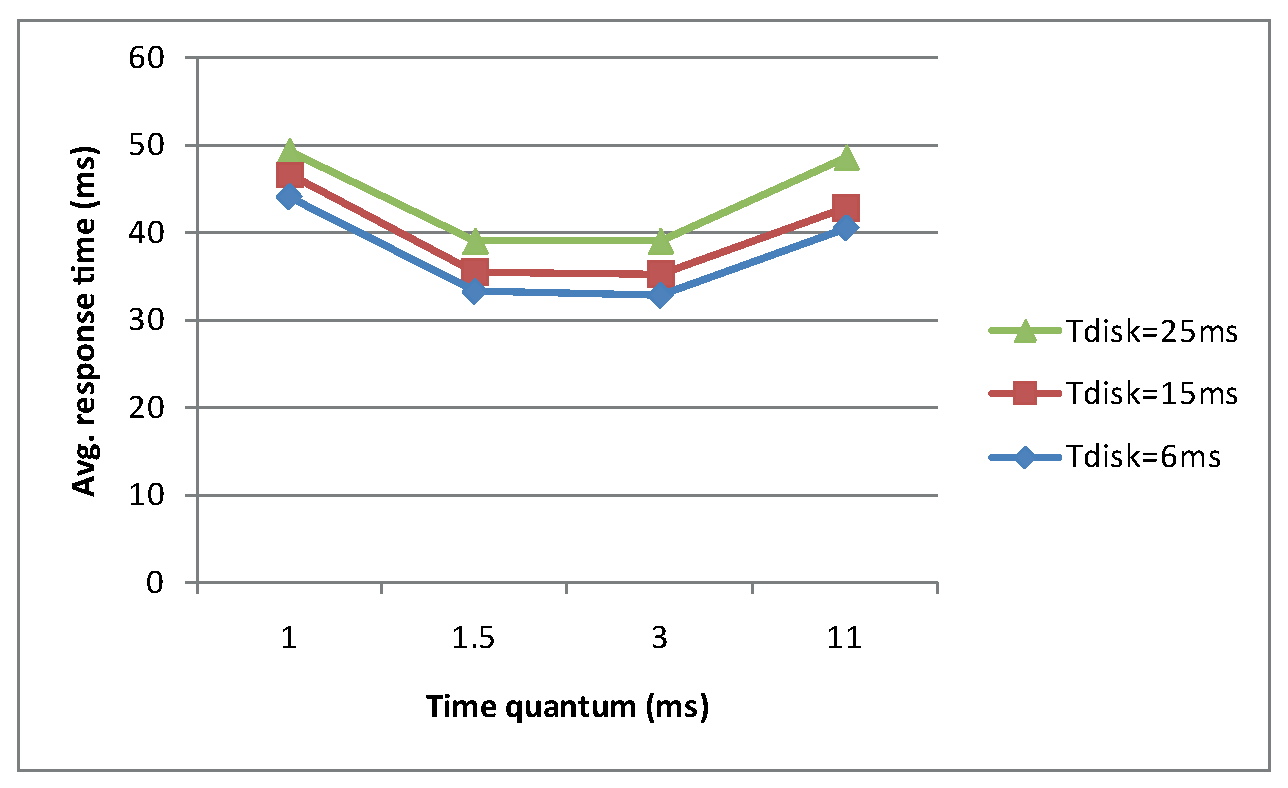
\includegraphics[width=0.8\textwidth]{responseTime.eps}
\caption{Impact on response time}
\end{center}
\end{figure}

From Figure 1, we can see that the optimal time quantum to shorten response time is somewhere between 1 ms and 1.5 ms. Too short or too long time quantum values would both hurt the responsiveness of the interactive processes (Process 0 through 8 in this paper). The reason is as follows.

\begin{itemize}
\item For too short time quantum values such as 1 ms, even the shortest process needs to get the CPU twice to finish, which means waiting for each of the other processes getting and yielding CPU.
\item For too long time quantum values such as 11 ms, although short processes can finish their jobs by getting CPU for just one time, before they can execute for the next time, they need to wait for long processes (Process 9 in this paper) using CPU for full time quanta.
\end{itemize}

\begin{figure}[h]
\begin{center}
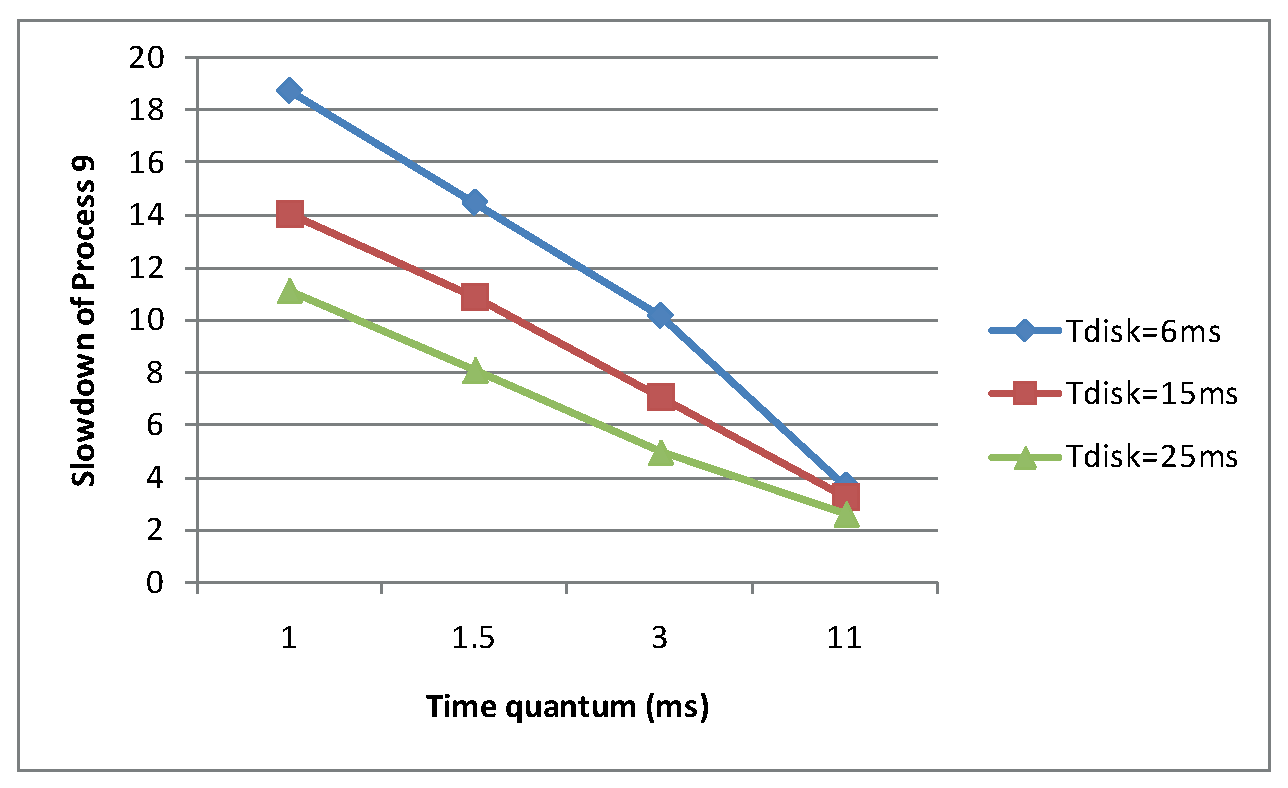
\includegraphics[width=0.8\textwidth]{slowdown.eps}
\caption{Impact on slowdown}
\end{center}
\end{figure}

From Figure 2, we can see that the slowdown drops consistently as time quantum goes up, no matter how long the disk operation takes. It is because the longer the time quantum, the less times the long processes need to get the CPU to finish. 

On the other hand, faster disk causes larger slowdown, because the faster the disk, the faster the short processes come back to ready queue, so the long processes have less chances to continuously get two or more CPU time quanta in a row.

\begin{figure}[h]
\begin{center}
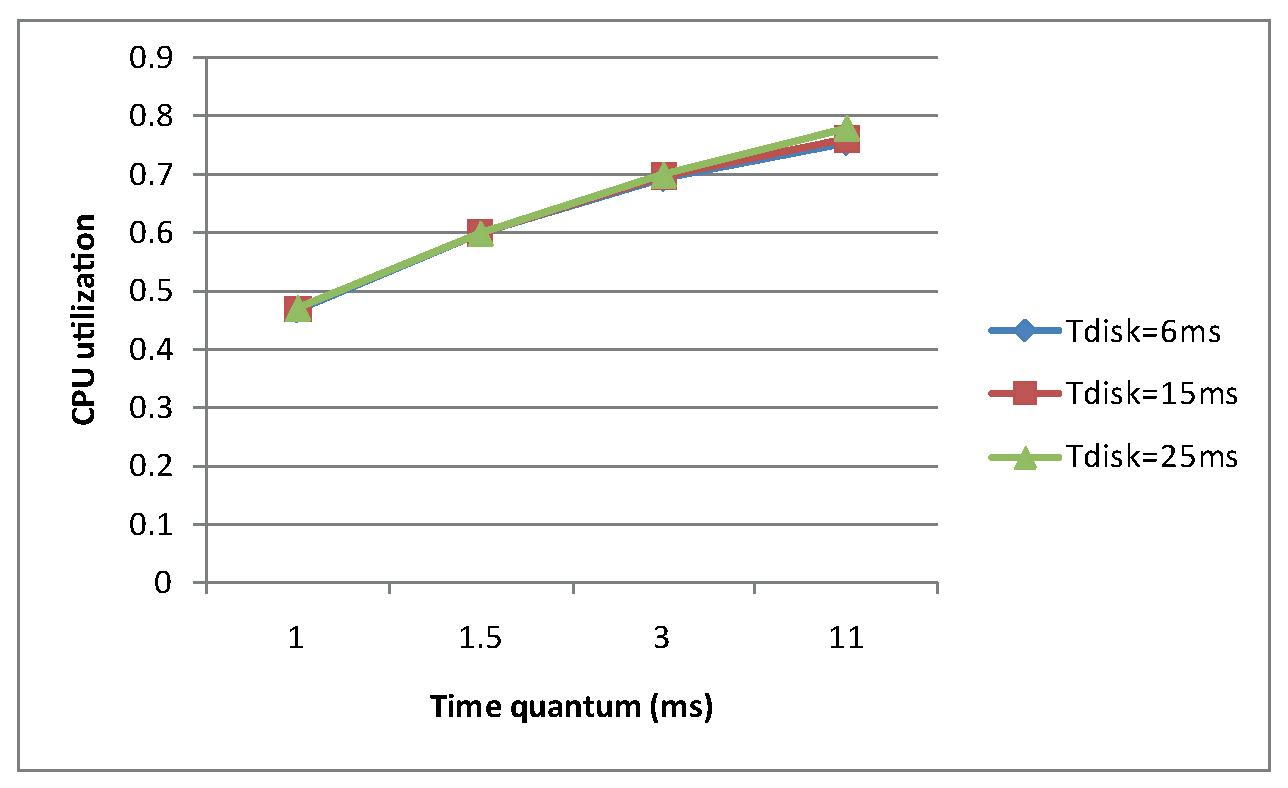
\includegraphics[width=0.8\textwidth]{cpuUtil.eps}
\caption{Impact on CPU utilization}
\end{center}
\end{figure}

From Figure 3, we can see that the CPU utilization increases consistently as time quantum goes up, no matter how long the disk operation takes, and the disk speed does not influence CPU utilization much. It is because the longer the time quantum, the less fraction of the CPU time is spent on context switching. So long as the disk is not so slow as to create long CPU idle time (when all the processes are doing IO, the CPU is idle), disk speed does not influence the CPU utilization.

\begin{figure}[h]
\begin{center}
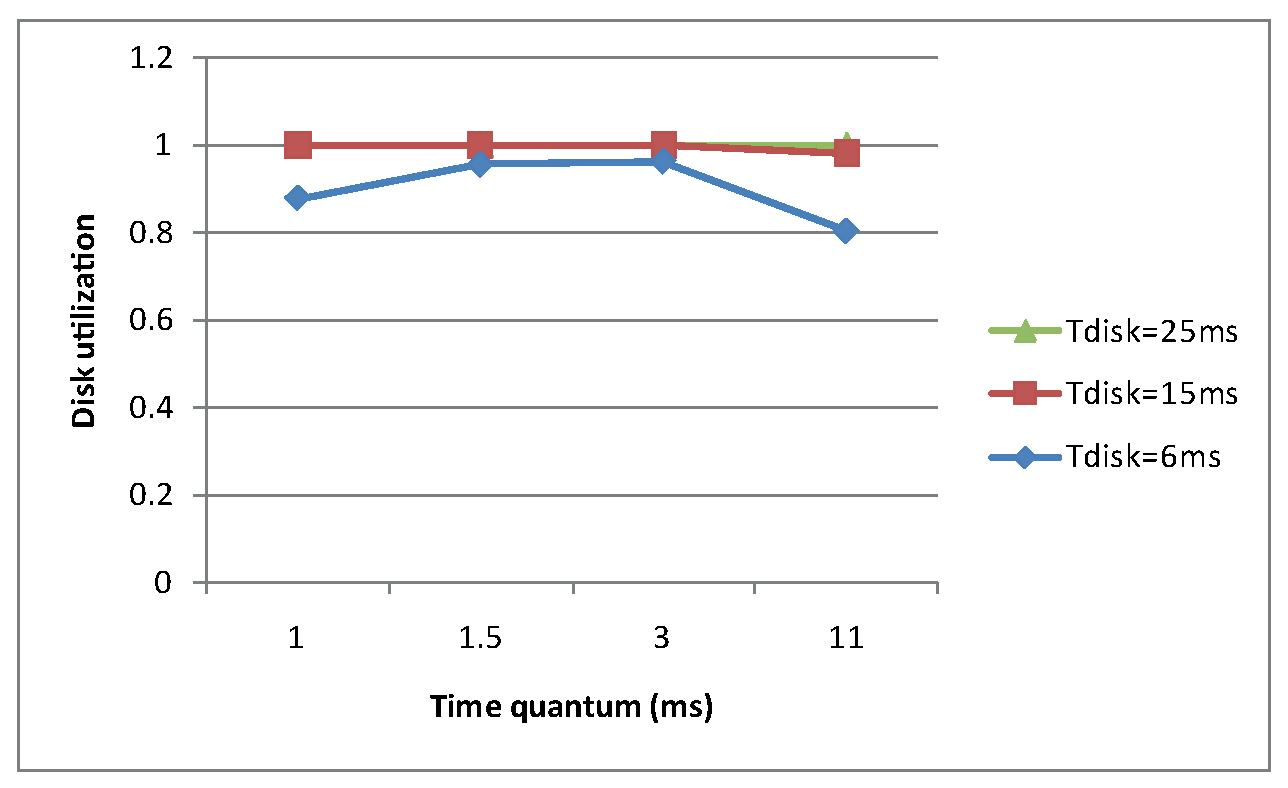
\includegraphics[width=0.8\textwidth]{diskUtil.eps}
\caption{Impact on disk utilization}
\end{center}
\end{figure}

From Figure 4, we can see the following results.

\begin{itemize}
\item for fast disk, the time quantum for the best disk utilization is somewhere between 1 ms and 1.5 ms, too short or too long time quantum lengths both lower the disk utilization. Because if the time quantum is too short, all the processes have to yield and get CPU for multiple times before they can perform IO operations, rendering much disk idle time; if the time quantum is too long, short processes have to wait, after finishing their IO operations, in the ready queue for the long processes using CPU. This also cause disk idle time.
\item for slow disk, the time quantum does not influence the disk utilization much if it is not much longer than an IO operation time. Because in this case some of the short processes are still doing IO operations when the long processes finish using the CPU, so the disk is always busy.
\end{itemize}

\end{document}

